\documentclass[5p,twocolumn]{elsarticle}

\usepackage{lineno,hyperref}
\usepackage{amsmath}% http://ctan.org/pkg/amsmath
\usepackage{bm}
\usepackage{multirow}
\usepackage{float}
\modulolinenumbers[5]

\journal{Journal of \LaTeX\ Templates}

%%%%%%%%%%%%%%%%%%%%%%%
%% Elsevier bibliography styles
%%%%%%%%%%%%%%%%%%%%%%%
%% To change the style, put a % in front of the second line of the current style and
%% remove the % from the second line of the style you would like to use.
%%%%%%%%%%%%%%%%%%%%%%%

%% Numbered
%\bibliographystyle{model1-num-names}

%% Numbered without titles
%\bibliographystyle{model1a-num-names}

%% Harvard
%\bibliographystyle{model2-names.bst}\biboptions{authoryear}

%% Vancouver numbered
%\usepackage{numcompress}\bibliographystyle{model3-num-names}

%% Vancouver name/year
%\usepackage{numcompress}\bibliographystyle{model4-names}\biboptions{authoryear}

%% APA style
%\bibliographystyle{model5-names}\biboptions{authoryear}

%% AMA style
%\usepackage{numcompress}\bibliographystyle{model6-num-names}

%% `Elsevier LaTeX' style
\bibliographystyle{elsarticle-num}
%%%%%%%%%%%%%%%%%%%%%%%

\begin{document}

\begin{frontmatter}

\title{Transient Inductive Interferences on a Pipeline due to Transmission Line Faults}


%% Group authors per affiliation:
\author{Caio M. Moraes\corref{UnB}, Amauri G. Martins-Britto, Felipe V. Lopes, Kleber M. Silva}
\cortext[UnB]{Corresponding author}
\ead{www.elsevier.com}
\address{University of Brasília}


%%% or include affiliations in footnotes:
%\author[mymainaddress,mysecondaryaddress]{Elsevier Inc}
%\ead[url]{www.elsevier.com}
%
%\author[mysecondaryaddress]{Global Customer Service\corref{mycorrespondingauthor}}
%\cortext[mycorrespondingauthor]{Corresponding author}
%\ead{support@elsevier.com}
%
%\address[mymainaddress]{1600 John F Kennedy Boulevard, Philadelphia}
%\address[mysecondaryaddress]{360 Park Avenue South, New York}

\begin{abstract}
Electromagnetic interferences (EMI) in shared right-of-ways between transmission lines (TLs) and nearby metallic installations are increasing due to development of restricts regulations regarding the use of space. Whenever it happens, transient effects on TLs raise the voltage and current levels on the energized conductors and, consequently, it can present risks to the people and facilities involved. In this paper is presented an EMTP-based implementation of a circuit model which considers wave propagation in high frequencies intended to predict fault transients inductive coupling interferences in a shared right-of-way composed of a 88 kV power line. Proposed model is used to study four types of faults and 2 types of switching surges on the TL and their coupling impacts in metallic facilities occupying the same right-of-way are evaluated. Results show that under line-to-ground transient conditions the coupling impacts are the worsts of all fault types for the system. Furthermore, unbalance factor of current and voltage in TL for each type of fault is calculated, showing that to arise of current unbalance there is an arise of maximum transient induced voltage on pipeline and to arise of voltage and current unbalance influences in a greater steady-state induced voltage after fault conditions. In capacitor bank switching surges, results presents that the induced voltage is influenced by capacitive coupling and has an exponential decay behavior.   
\end{abstract}

\begin{keyword}
Electromagnetic interferences, EMTP/ATP, inductive coupling, pipelines and transmission lines.
\end{keyword}

\end{frontmatter}

\linenumbers

\section{Introduction}

Due to the development and industrialization of cities, the loading levels of transmission lines (TLs) have become higher. These structures are exposed to several types of electromagnetic transients (EMTs) that increase the voltage and current levels above the nominal values, such as: short circuits, atmospheric discharges, reconnections, energization, etc. 

The effects caused by EMTs on power lines affect the operation and can generate risks to this installation. In addition, these effects also generate risks to metallic structures neighboring the transmission lines through three types of electromagnetic interference (EMI): inductive, conductive and capacitive coupling \cite{CIGREWG36}.



Among the EMTs on TLs, occurrence of faults are the most common. These are an unavoidable EMT due to the fact it is caused by natural events, which is uncontrollable by human beings.The TL fault is mainly classified into four type of faults depending on it is characteristics and the engagement of soil. The appropriate percentage of different phase currents, the maximum and minimum occurrence of various types of faults are given by \cite{Nithyavelam2018}:

\begin{itemize}
	\item Single line-to-ground fault: 70 to 80\%
	\item Line-to-line to ground fault: 10 to 17\%
	\item Line-to-line fault: 8 to 10\%
	\item Three-phase fault: 3\% 
\end{itemize} 

In addiction to faults, switching surges are important to the design insulation in TL and impacts on cost of the project. Switching overvoltages occurs from maneuver of switching devices in the power system under normal operation conditions or due to result of fault clearings. The mainly switching maneuver is TL energization, reconnections, capacitor and reactor bank, occurrence of faults and circuit breakers opening \cite{Ibrahim2005,Hamza2019}.

Generally, power lines models considered in EMI studies due to EMT in TLs are composed of cascading $\pi$—cells, which being concentrated parameters. This line model is well-known to have limitations as it incorrectly represents wave propagation at TL and high frequency transient behaviors. The studies involving EMT interferences in the literature considers simplified right-of-ways, representing the path just as parallelisms between the facilities, which not represents the shared right-of-ways in real world. Also, these documents present just a line-to-ground fault in TL, neglecting the other type of faults \cite{Christoforidis2003,Qi2013,Wu2017,Alexandru2020}.  

In  order  to  produce  a  more  realistic  and  complete study  for  EMI due to transients in TLs,  this  paper presents an EMTP-type implementation of a circuit model that considers wave propagations in high frequency intended to study transient inductive coupling in a power distribution line and case of right-of-way sharing with other facilities. The right-of-way is composed of parallelism, obliquities and one crossing which is a good sample of a real shared right-of-way. 

The proposed model is used to study mainly types of EMT and its inductive coupling interferences in the pipeline are evaluated.

Of practical relevance to several power companies, as well as industries that use pipeline transportation systems, this work is expected to contribute with an implementation of a simple and precise circuit model for studies of inductive coupling phenomena under nominal load and transients regime, suitable for handling realistic geometries of transmission lines and pipelines in shared right-of-ways.

\section{System under study}

Simplified single-line diagram with geometry of the shared right-of-way is given in Fig. \ref{fig:EMIzone}, which $Z_{A,0} = j0.191$, $Z_{A,+} = j0.0654$ and $Z_{B,0} = j0.1908$, $Z_{B,+} = j0.0654$ in ohms per meter. 

\begin{figure}[h]
	\begin{center}
		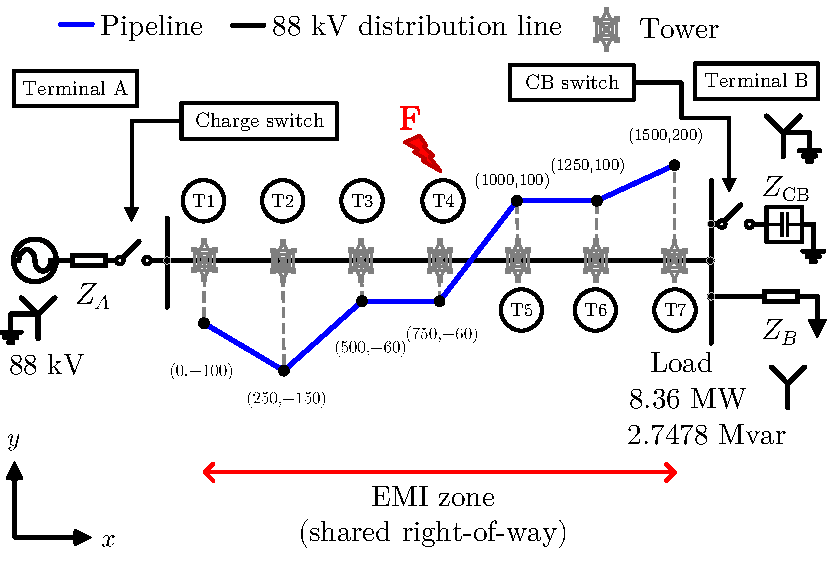
\includegraphics[width=8.4cm]{img/sys_88_top.pdf}    % The printed column width is 8.4 cm.
		\caption{Simplified single-line diagram and geometry of EMI zone, adapted from \cite{Martins-Britto2020}.} 
		\label{fig:EMIzone}
	\end{center}
\end{figure}

The charge and capacitor bank (CB) switch are used only in energization and CB switching study, respectively. 

As shown in Fig. \ref{fig:EMIzone}, the EMI zone has approximately 1.5 kilometers of extension. The EMI zone is composed of an untransposed single-circuit distribution line, horizontal configuration containing two shield wires, as shown in Fig. \ref{fig:TowerGeometry}. At nominal load conditions, the 88 kV distribution line is energized with 90 A per phase, ABC sequence and 60 Hz frequency. The substation at Terminal A is grounded through 1 $\Omega$ resistance. 

\begin{figure}[h]
	\begin{center}
		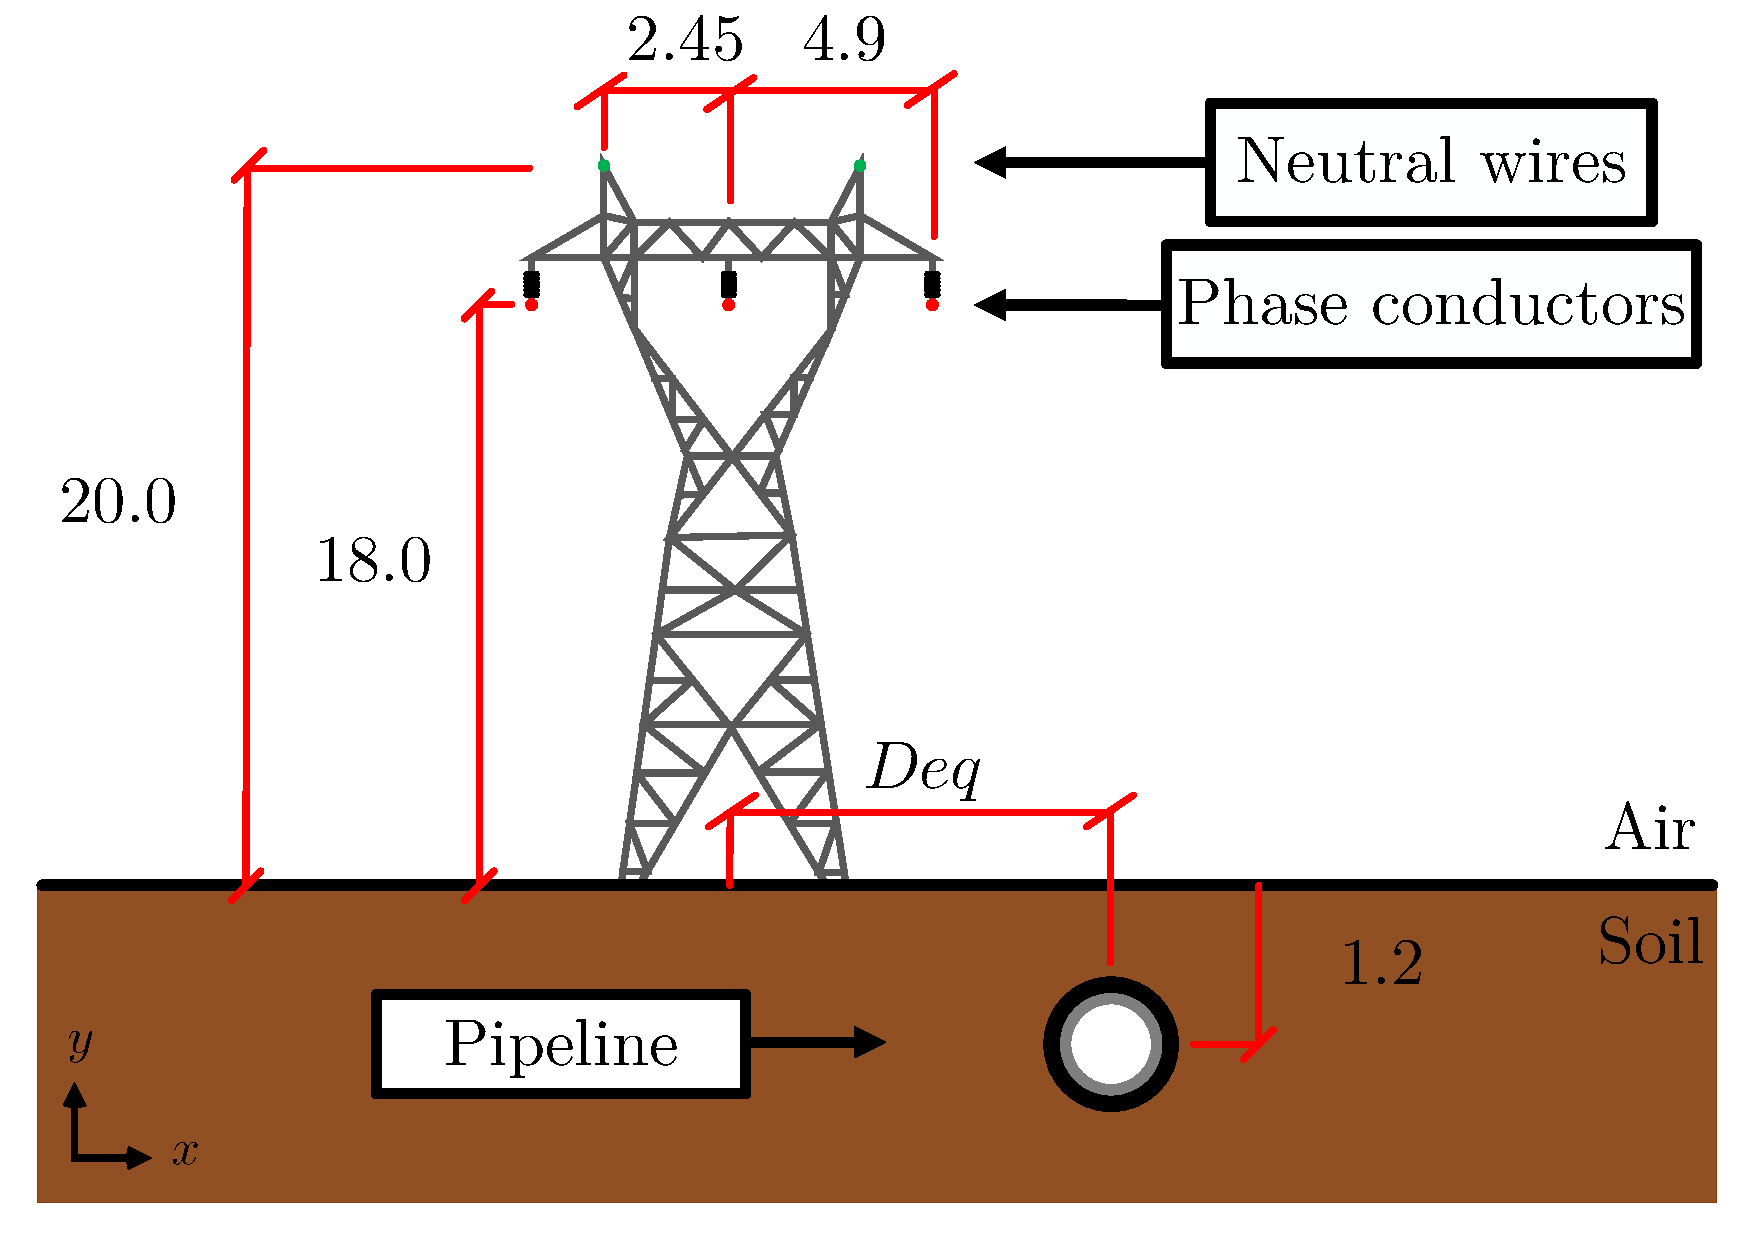
\includegraphics[width=8.4cm]{img/TowerGoemetry.pdf}    % The printed column width is 8.4 cm.
		\caption{Distribution line tower geometry.} 
		\label{fig:TowerGeometry}
	\end{center}
\end{figure}

A 14" diameter carbon-steel pipeline shares the same right-of-way of the distribution line. The pipeline is positioned buried at 1.2 meters and it is grounded at the terminals through resistances equal to 10 $\Omega$.  Physics characteristics of the conductors and 14" pipe are summarized in Tab.\ref{tab:ConductorsCharacteristics}.

The soil model is represented by a uniform resistivity value equal to 100 ohms-meter.

\begin{table}[h]
	\centering
	\caption{Specification and characteristics of system conductors}
	\footnotesize
	\begin{tabular}{cccc}
		\textbf{Conductor}         & \textbf{\boldmath{$r_{out}$ [m]}} & \textbf{\boldmath{$r_{in}$ {[}m{]}}} & \textbf{\boldmath{$R_{DC}${[}$\Omega/km${]}}} \\ \hline
		{ACSR Grosbeak}     & 0.0125705                        & 0.0046355                        & 0.0924806                          \\
		{Steel 3/8" EHS-CG} & 0.004572                         & -                                & 3.42313                            \\
		{Pipe 14"}          & 0.1778                           & 0.168275                         & 0.099516                          \\ \hline
	\end{tabular}
	\label{tab:ConductorsCharacteristics}
\end{table}

\section{Equivalent circuit model}

Pipeline is subdivided in coupling regions of parallel sections with the TL. These coupling regions are modeled using equivalent length and distance calculated from approximations and crossings between the facilities in shared right-of-way, as described in detain in \cite{Moraes2020}.

Each coupling region is constructed in EMTP/ATP software using Line/Cable Constants (LCC) objects, which execute the inductive coupling calculations \cite{Martins-Britto2020}. Parameters of TL conductors and pipeline are calculated using Bergeron model, which considers high frequency wave propagation on conductors. The equivalent circuit model construction methodology is thoroughly discussed in references \cite{Martins-Britto2020,Moraes2020,Martins-Britto2021}.



\section{Nominal load study}

Under nominal load conditions, the TL operates in 88 kV and 90 A per phase considering charge switch closed and CB switch open, as shown in Fig \ref{fig:NLindVoltageTL}.

The induced voltage a long time in pipeline extremities and nearby crossing location are presented in Fig. \ref{fig:NLindVoltage3plots}. 

Fig. \ref{fig:NLindVoltage} shows the induced voltage in the pipeline along EMI zone considering the distribution line under nominal conditions of load. 

The proposed model presents 6.5\% RMS deviation compared with a software widely regarded as the industry-standard for EMI studies. Others systems using the proposed to predict induced voltage are reported in \cite{Moraes2020,Martins-Britto2021}, presenting less than 10\% RMS error.

The induced voltage reaches its maximum value at crossing with the TL and decreases in magnitude as moves towards the terminals of the pipeline, as shown in Fig. \ref{fig:NLindVoltage3plots} and \ref{fig:NLindVoltage}. An asymmetrical distribution is observed due to the fact the coupling regions after and before crossing point has distinct obliquities and, consequently, different parallel equivalent lengths, although same grounding resistance is considered at both ends. 

\begin{figure}[h]
	\begin{center}
		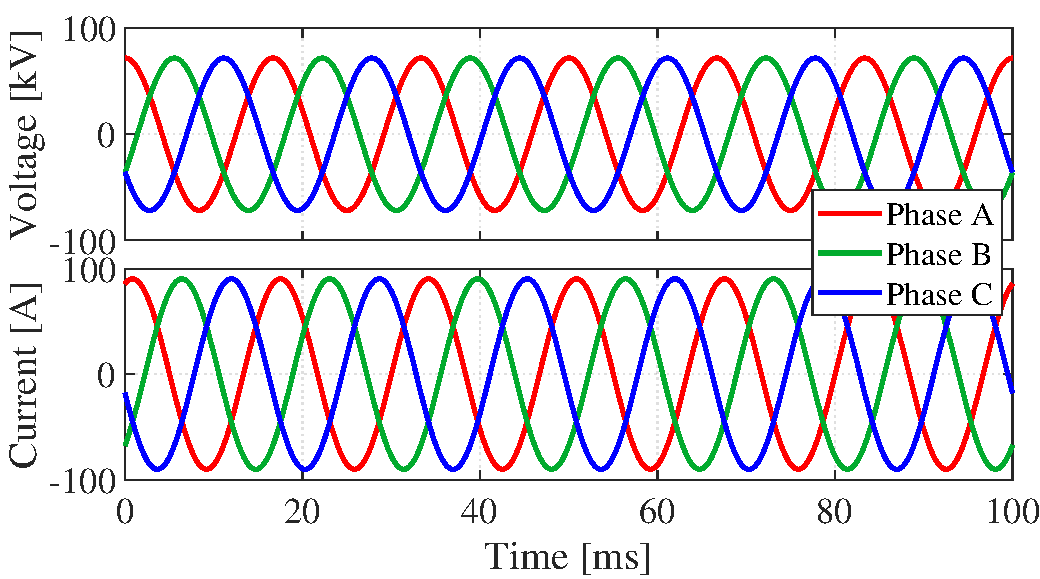
\includegraphics[width=8.4cm]{img/NLindVoltage_TL.pdf}    % The printed column width is 8.4 cm.
		\caption{Transmission line current and voltage under nominal load conditions.} 
		\label{fig:NLindVoltageTL}
	\end{center}
\end{figure}

\begin{figure}[h]
	\begin{center}
		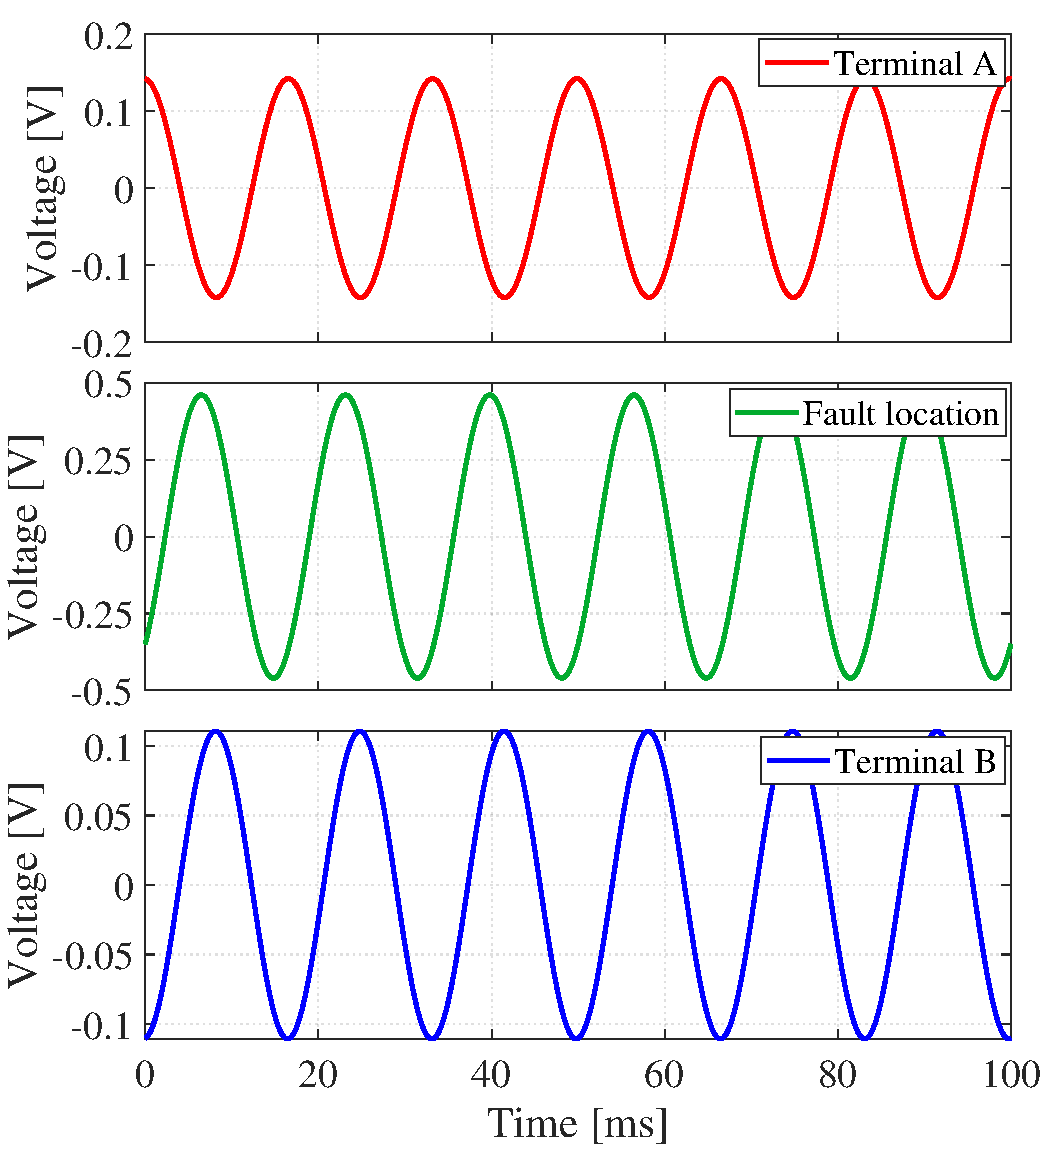
\includegraphics[width=8.4cm]{img/NLindVoltage_3plots.pdf}    % The printed column width is 8.4 cm.
		\caption{Pipeline induced voltage in nominal load regime.} 
		\label{fig:NLindVoltage3plots}
	\end{center}
\end{figure}

\begin{figure}[h]
	\begin{center}
		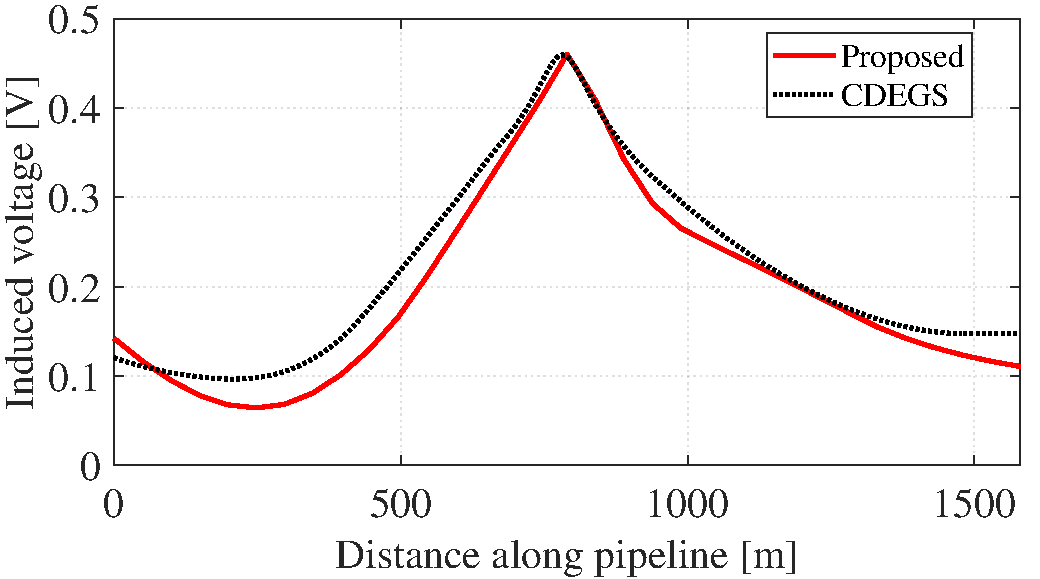
\includegraphics[width=8.4cm]{img/NLindVoltage.pdf}    % The printed column width is 8.4 cm.
		\caption{Induced voltage along pipeline in nominal load regime.} 
		\label{fig:NLindVoltage}
	\end{center}
\end{figure}

\section{Transient fault study}

Intersection of the facilities occurs between towers \#4 and \#5. Four types of fault (A-g, AB, AB-g and ABC) are simulated in tower \#4 in order to study the influence of fault transients on inductive coupling between pipeline and TL. The tower \#4 is chosen because it is closest to the crossing point. Line-to-ground and line-to-line fault resistances are considered $R_{F} = 0.00001$ $\Omega$, to represent a short circuit between phases or phase to ground.

In this type of study is aimed to observe just fault interferences. In other words, the system is considered with charge switch closed permanently and CB is out of operation. 

\subsection{Single line-to-ground fault}

A single line-to-ground fault is applied to TL between phase A to ground through $R_{F}$ resistance, as shown in Fig. \ref{fig:AGindVoltageTL}. 

\begin{figure}[h]
	\begin{center}
		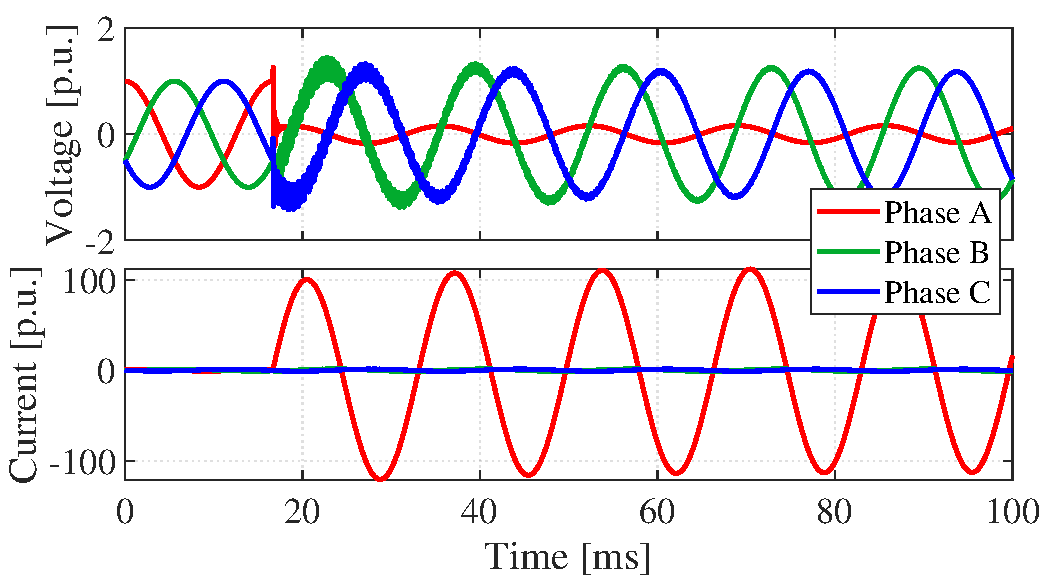
\includegraphics[width=8.4cm]{img/AGindVoltage_TL.pdf}    % The printed column width is 8.4 cm.
		\caption{Transmission line current and voltage in A-g fault regime.} 
		\label{fig:AGindVoltageTL}
	\end{center}
\end{figure} 

In Fig. \ref{fig:AGindVoltage} are shown the steady-state induced voltage after fault and the maximum transient induced voltage value along pipeline path.

\begin{figure}[h]
	\begin{center}
		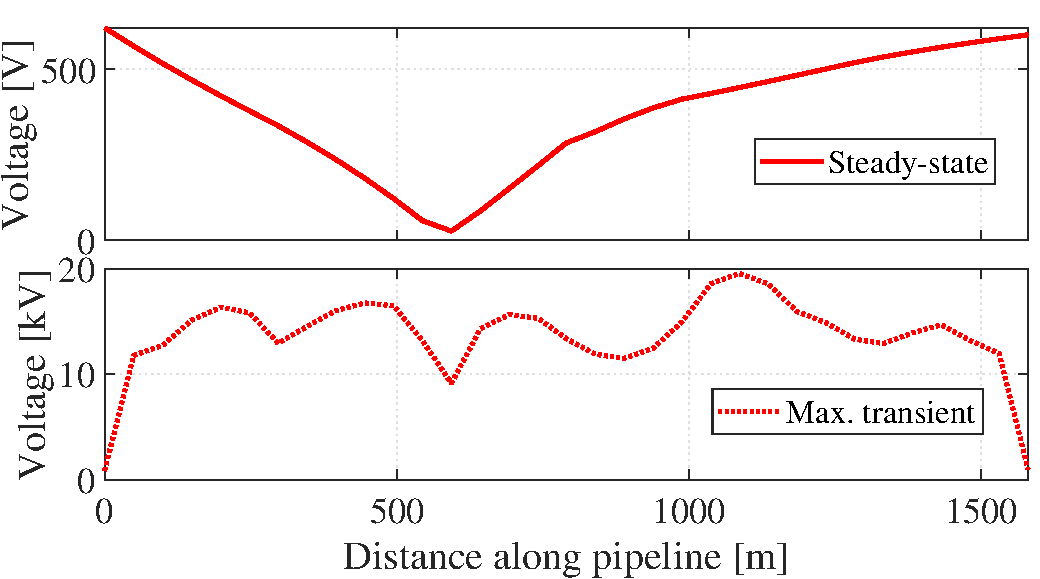
\includegraphics[width=8.4cm]{img/AGindVoltage.pdf}    % The printed column width is 8.4 cm.
		\caption{Steady-state induced voltage and maximum induced voltage along pipeline in A-g fault regime.} 
		\label{fig:AGindVoltage}
	\end{center}
\end{figure}

The induced voltages a long time at pipeline terminals and nearby fault location are presented in Fig. \ref{fig:AGindVoltage3plots}.

\begin{figure}[H]
	\begin{center}
		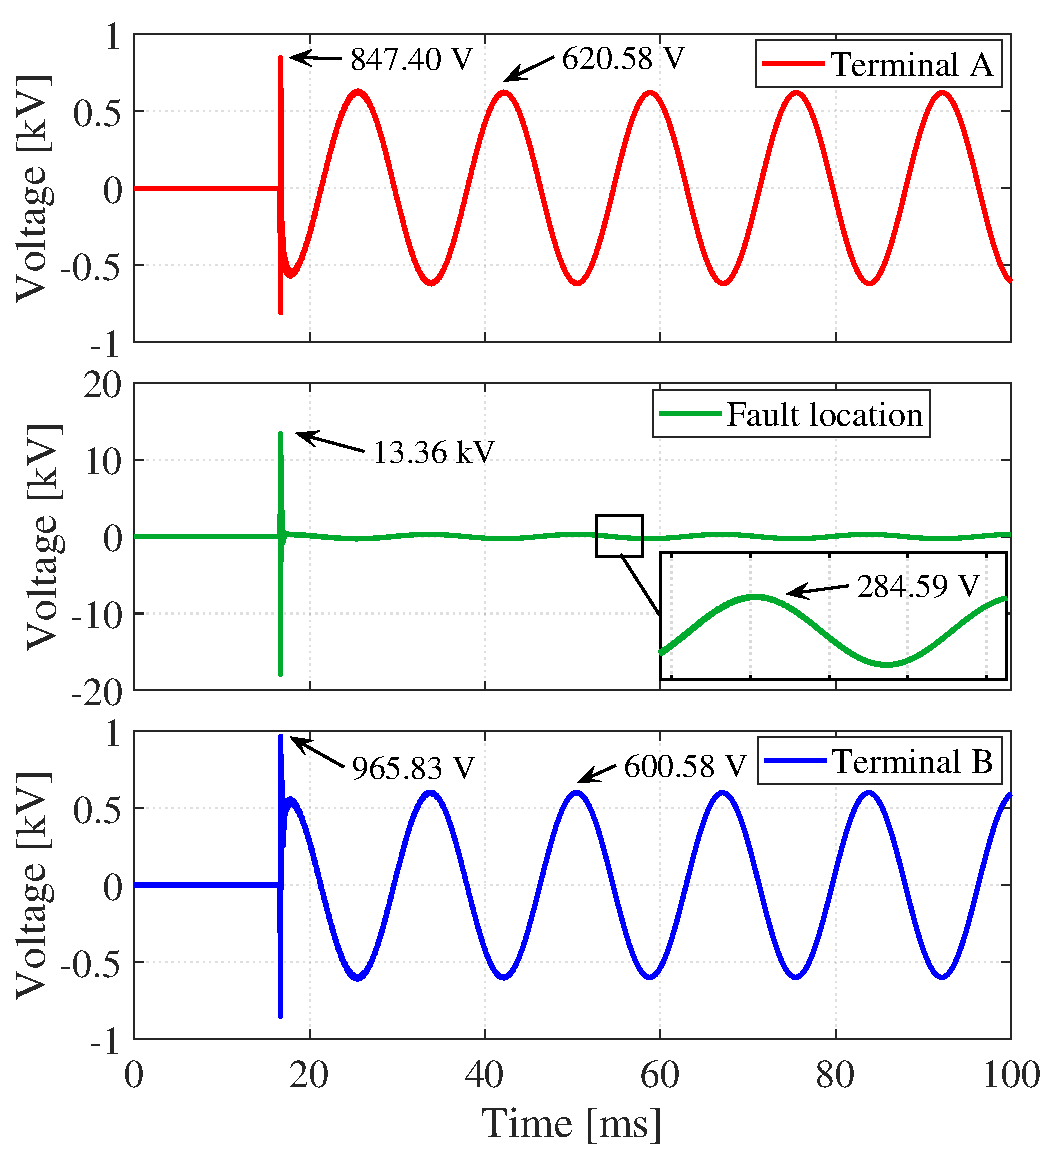
\includegraphics[width=8.4cm]{img/AGindVoltage_3plots.pdf}    % The printed column width is 8.4 cm.
		\caption{Induced voltage \textit{versus} time at Terminal A, Terminal B and nearby fault location to A-g fault.} 
		\label{fig:AGindVoltage3plots}
	\end{center}
\end{figure}



For single line-to-ground fault, the induced voltage has reflected behavior at pipeline extremities, as shown in Fig. \ref{fig:AGindVoltage3plots}. The steady-state induced voltage reaches 500 V and the maximum transient reaches 20 kV due to current in TL arises to 100 times the nominal load conditions in phase A. The minimum value of steady-state induced voltage is observed at nearby fault location due to the fact the resulting electromagnetic field in that point owing to currents flowing from phases to shield wires is approximately zero and reaches its maximum value towards pipeline terminals. However, the maximum transients induced voltage has its minimum value at pipeline extremities due to the grounding resistances at Terminal A and B.

\subsection{Line-to-line fault}

For line-to-line fault, is considered an $R_{F}$ resistance between phase A and B. Current and voltage in TL due to AB fault is presented in Fig. \ref{fig:ABindVoltageTL}.

\begin{figure}[h]
	\begin{center}
		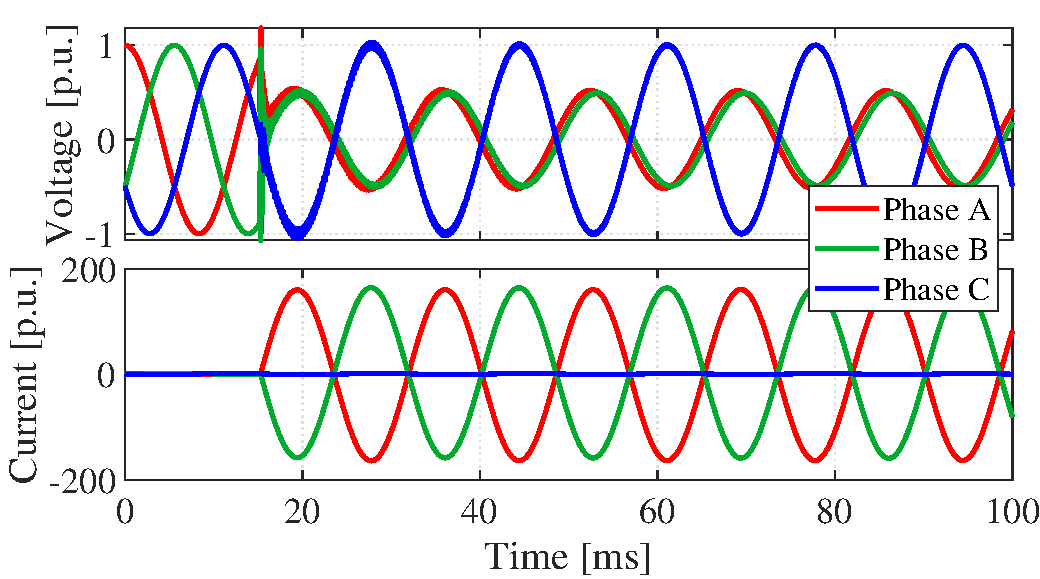
\includegraphics[width=8.4cm]{img/ABindVoltage_TL.pdf}    % The printed column width is 8.4 cm.
		\caption{Transmission line current and voltage in AB fault regime.} 
		\label{fig:ABindVoltageTL}
	\end{center}
\end{figure}

Current in TL after the line-to-line fault arises to 163 p.u., this causes a maximum induced voltage equal a 3.06 kV, as shown in Fig. \ref{fig:ABindVoltage}. In spite of higher currents in TL, the induced voltages are lower than in single line-to-ground due to its more balanced fault, generating a lower resulting electromagnetic field on a pipeline.   

\begin{figure}[h]
	\begin{center}
		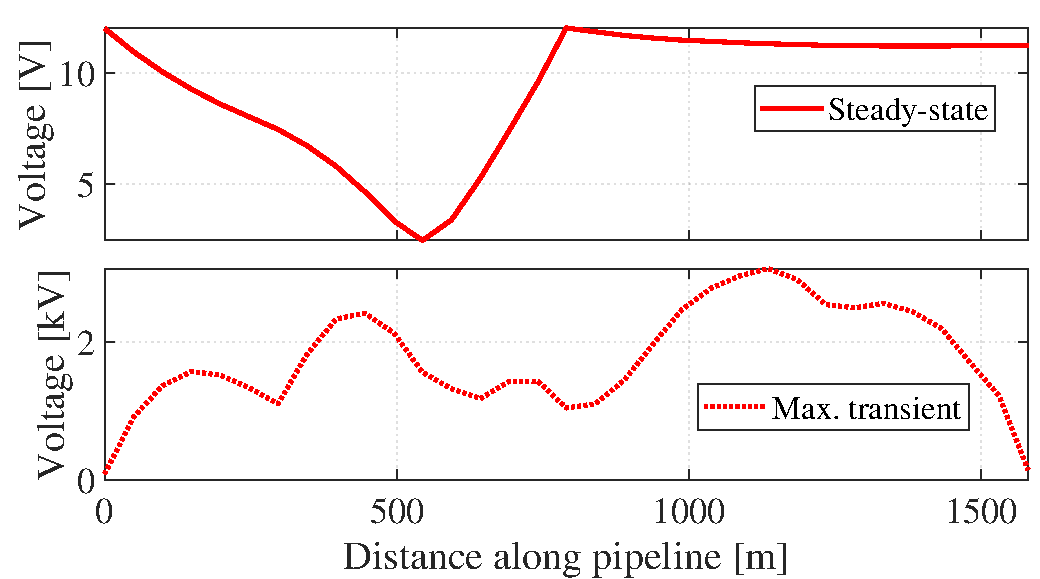
\includegraphics[width=8.4cm]{img/ABindVoltage.pdf}    % The printed column width is 8.4 cm.
		\caption{Steady-state induced voltage and maximum induced voltage along pipeline in AB fault regime.} 
		\label{fig:ABindVoltage}
	\end{center}
\end{figure}

Fig. \ref{fig:ABindVoltage3plots} shows that there is a peak in the instant of occur fault and its reduce over time at the particular points analyzed. At Terminals A and B induced voltage are similar in terms of magnitude and behavior, though mirrored on account of wave propagation. 

\begin{figure}[H]
	\begin{center}
		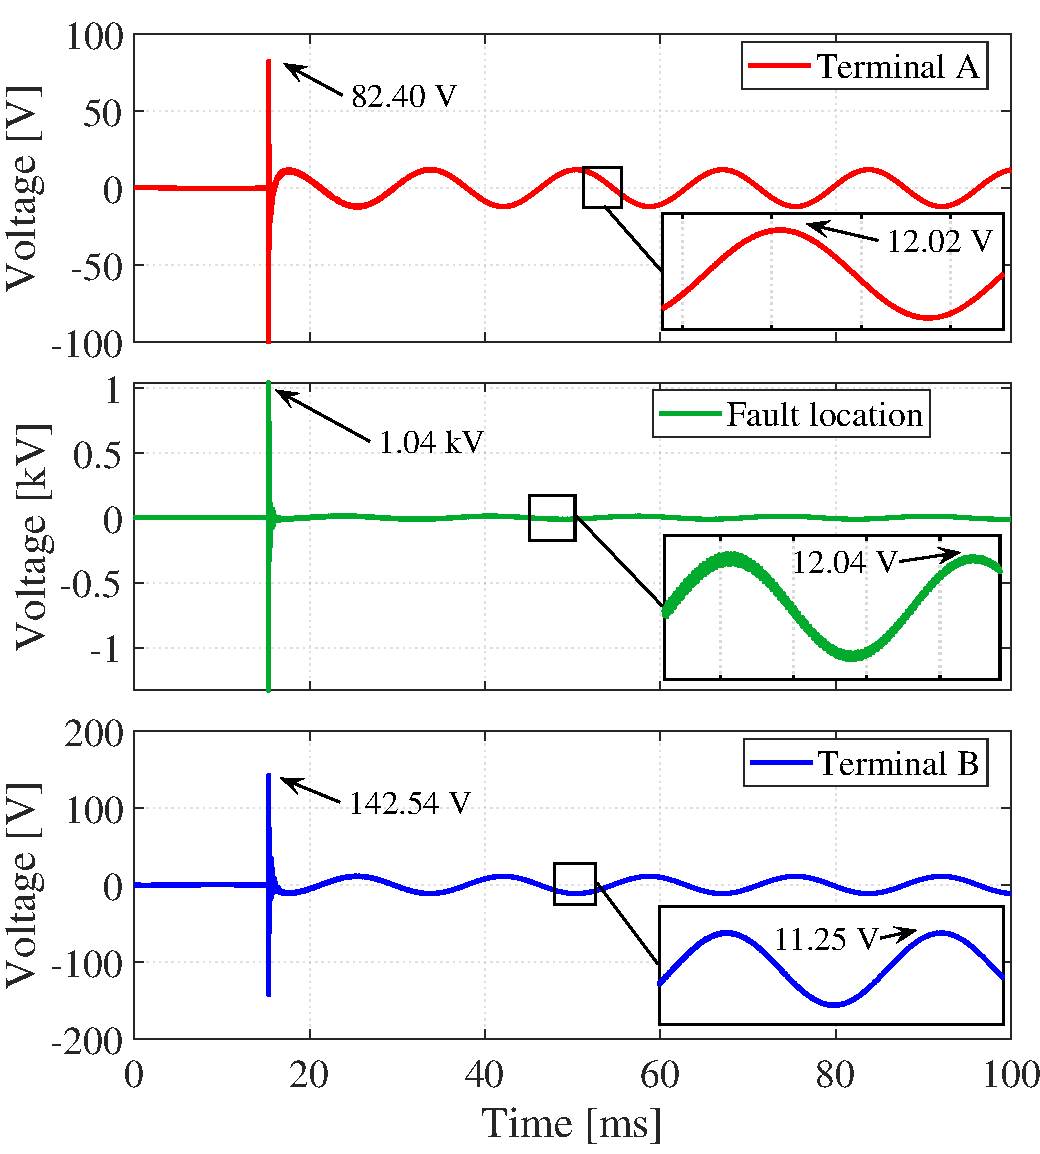
\includegraphics[width=8.4cm]{img/ABindVoltage_3plots.pdf}    % The printed column width is 8.4 cm.
		\caption{Induced voltage \textit{versus} time at Terminal A, Terminal B and nearby fault location to AB fault.} 
		\label{fig:ABindVoltage3plots}
	\end{center}
\end{figure}

\subsection{Line-to-line to ground fault}

In this case, a $R_{F}$ resistance is connected between phase A and B with another $R_{F}$ resistances connecting the faulted phases in ground. Fig. \ref{fig:ABGindVoltageTL} present current and voltage in TL for AB-g fault.

\begin{figure}[h]
	\begin{center}
		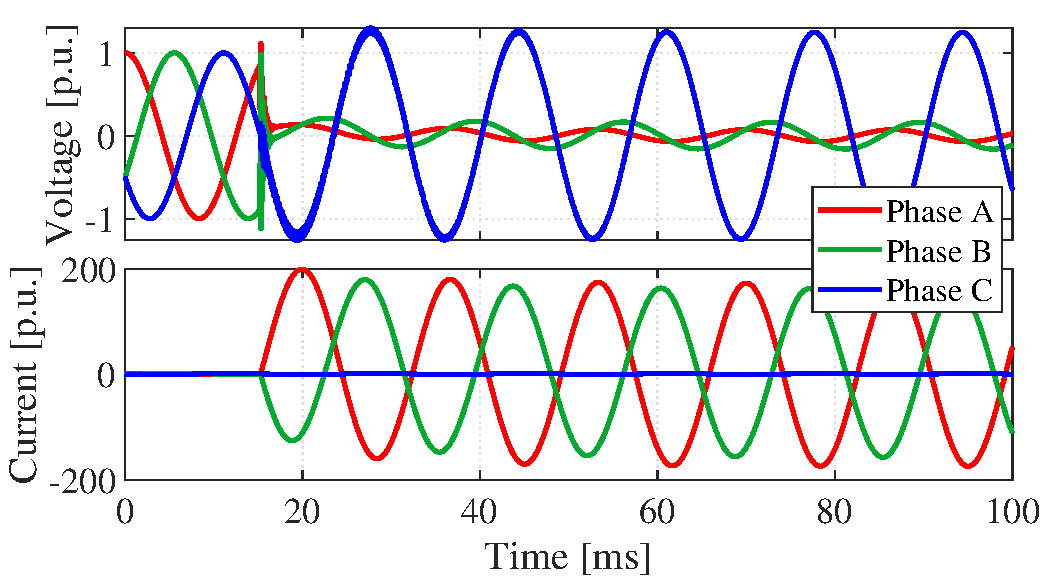
\includegraphics[width=8.4cm]{img/ABGindVoltage_TL.pdf}    % The printed column width is 8.4 cm.
		\caption{Current and voltage waveforms at Terminal A for AB-g fault regime.} 
		\label{fig:ABGindVoltageTL}
	\end{center}
\end{figure}

In line-to-line to ground fault the current and maximum transient in induced voltage are similar to line-to-line fault, though the steady-state induced voltage behavior is closest to observed in line-to-ground fault, as presented in Fig. \ref{fig:ABGindVoltage}. Possibly, this profile is observed due to faults involving ground arises voltage difference between faulted phases and phases operating normally. The greatest phase unbalance generates higher currents on the pipeline in steady-state regime after fault involving the soil.    

\begin{figure}[h]
	\begin{center}
		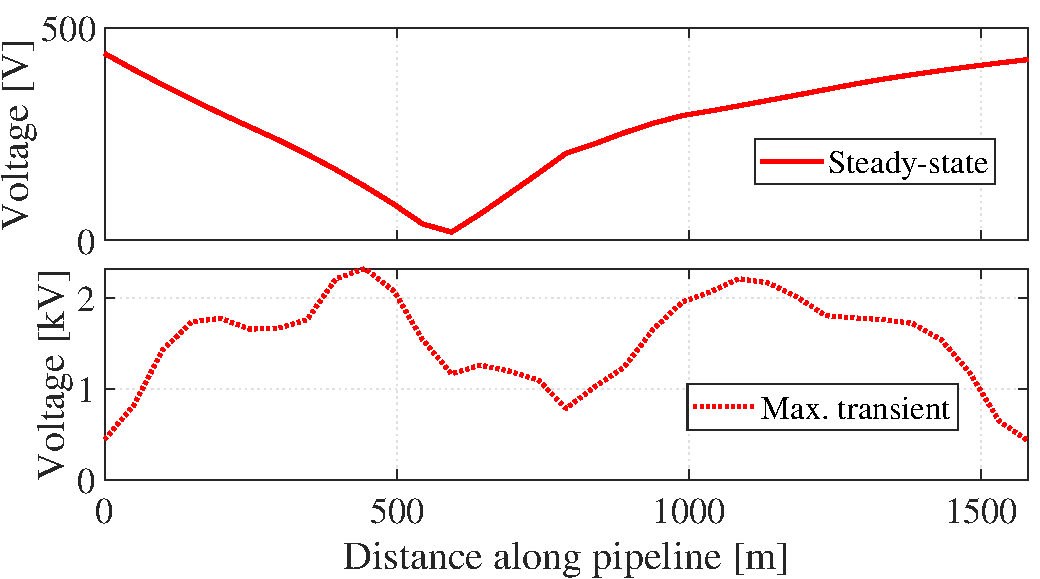
\includegraphics[width=8.4cm]{img/ABGindVoltage.pdf}    % The printed column width is 8.4 cm.
		\caption{Steady-state induced voltage and maximum induced voltage along pipeline in AB-g fault regime.} 
		\label{fig:ABGindVoltage}
	\end{center}
\end{figure}

In induced voltage at terminals are not verified the peak in instant of fault occurrence, though as the other fault types. Fig. \ref{fig:ABGindVoltage3plots} shows this phenomenon. 

\begin{figure}[h]
	\begin{center}
		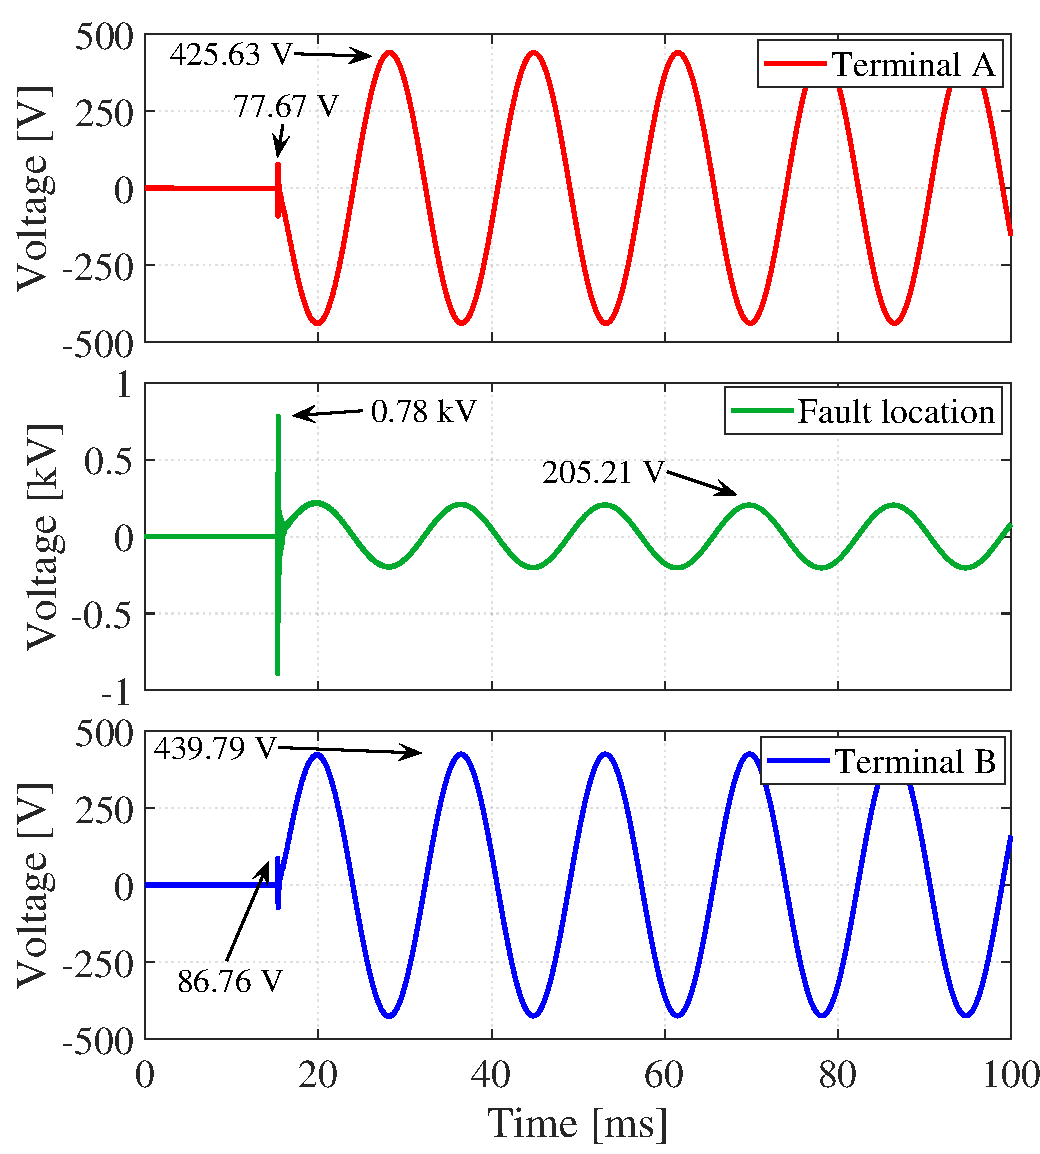
\includegraphics[width=8.4cm]{img/ABGindVoltage_3plots.pdf}    % The printed column width is 8.4 cm.
		\caption{Induced voltage \textit{versus} time at Terminal A, Terminal B and nearby fault location to AB-g fault.} 
		\label{fig:ABGindVoltage3plots}
	\end{center}
\end{figure}

\subsection{Three-phase fault}

In this case, currents in TL had its higher values from all fault types, reaching 341 p.u. in phase B, as presented in Fig. \ref{fig:ABCindVoltageTL}. 

\begin{figure}[h]
	\begin{center}
		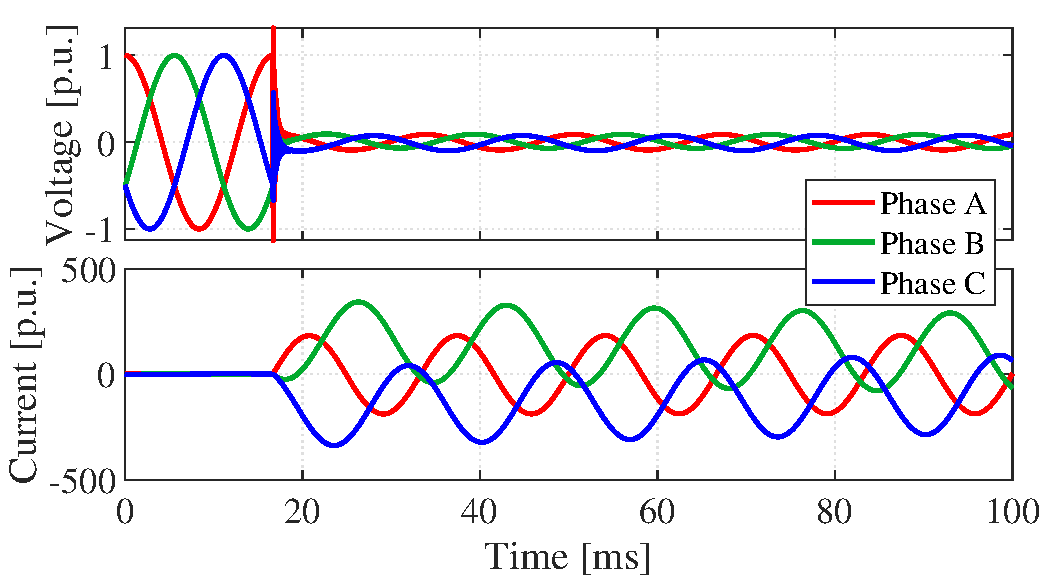
\includegraphics[width=8.4cm]{img/ABCindVoltage_TL.pdf}    % The printed column width is 8.4 cm.
		\caption{Current and voltage waveforms at Terminal A for ABC fault regime.} 
		\label{fig:ABCindVoltageTL}
	\end{center}
\end{figure}

For a fault not involving the ground, Fig. \ref{fig:ABCindVoltage} shows that ABC fault had the higher steady-state and maximum transient voltage values in the pipeline.   

An interesting fact is observed in Fig. \ref{fig:ABCindVoltage3plots}, this type of fault it is unique to not present voltage peaks in Terminal A and B of the pipeline.  

\begin{figure}[h]
	\begin{center}
		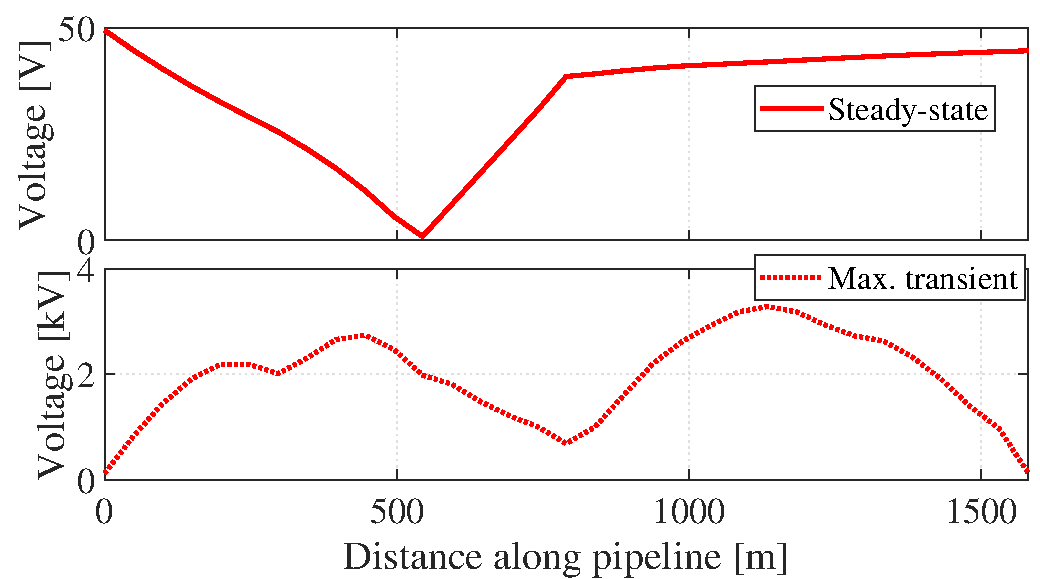
\includegraphics[width=8.4cm]{img/ABCindVoltage.pdf}    % The printed column width is 8.4 cm.
		\caption{Steady-state induced voltage and maximum induced voltage along pipeline in ABC fault regime.} 
		\label{fig:ABCindVoltage}
	\end{center}
\end{figure}

\begin{figure}[h]
	\begin{center}
		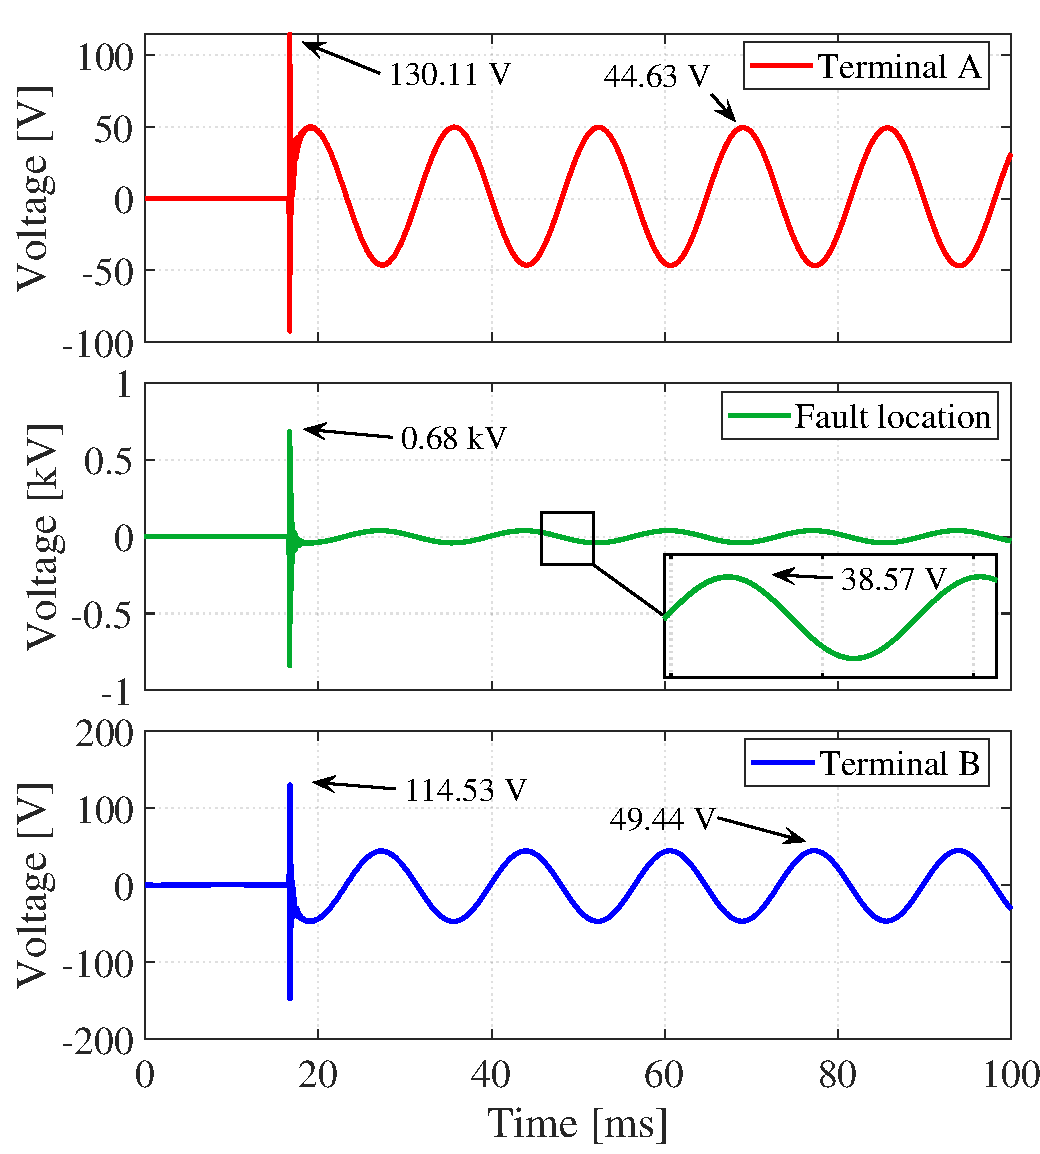
\includegraphics[width=8.4cm]{img/ABCindVoltage_3plots.pdf}    % The printed column width is 8.4 cm.
		\caption{Induced voltage \textit{versus} time at Terminal A, Terminal B and nearby fault location to ABC fault.} 
		\label{fig:ABCindVoltage3plots}
	\end{center}
\end{figure}

\subsection{Unbalance factor of fault transients}

In order to investigate a link between the induced voltage and the faulted current and voltage unbalance, an unbalance factor is calculated for each type of faulted described previously. The unbalance rate is defined in \cite{IEEE1993}, as following:

\begin{equation}
	K_{UR,\%} = \frac{\Delta K_{max}}{\overline{K}},
\end{equation}

\noindent in which $K$ represents voltage or current signal, $\Delta K_{max}$ is the maximum phase deviation from the average phase magnitude ($\overline{K}$), defined as:

\begin{equation}
	\overline{K} = \frac{K_{an} + K_{bn} + K_{cn}}{3}.
\end{equation}

Table \ref{tab:Unbalance} summarized the signals in TL and the pipeline for all types of faults studied and its related unbalance factor.


\begin{table*}[ht]
	\centering
	\caption{Outline of transients fault type interferences and unbalance factor}
	\footnotesize
	\begin{tabular}{ccccccccccccc}
		\textbf{}                            & \multicolumn{3}{c}{\textbf{Faulted Currents   {[}p.u.{]}}}                     & \multicolumn{3}{c}{\textbf{Faulted   Voltages {[}p.u.{]}}}                     & \multicolumn{2}{c}{\textbf{Ind.   Voltage {[}V{]}}} & \multicolumn{2}{c}{\textbf{Ind.   Voltage {[}\%{]}}} & \multicolumn{2}{c}{\textbf{Unb.   Factor {[}\%{]}}}              \\ \cline{2-13} 
		\multirow{2}{*}{\textbf{Fault Type}} & \multirow{2}{*}{\boldmath{$|I_{a}|$}} & \multirow{2}{*}{\boldmath{$|I_{b}|$}} & \multirow{2}{*}{\boldmath{$|I_{c}|$}} & \multirow{2}{*}{\boldmath{$|V_{a}|$}} & \multirow{2}{*}{\boldmath{$|V_{b}|$}} & \multirow{2}{*}{\boldmath{$|V_{c}|$}} & \textbf{Steady}         & \textbf{Max.}             & \textbf{Steady}         & \textbf{Max.}              & \multirow{2}{*}{\textbf{Current}} & \multirow{2}{*}{\textbf{Voltage}} \\
		&                          &                          &                          &                          &                          &                          & \textbf{State}          & \textbf{Transient}        & \textbf{State}          & \textbf{Transient}         &                                   &                                   \\ \hline
		\textbf{A-g}                         & 110.18                   & 1.32                     & 1.30                     & 0.16                     & 1.27                     & 1.20                     & 620.58                  & 19539.90                  & 1349.09                 & 42478.04                   & 289.57                            & 126.62                            \\
		\textbf{AB}                          & 159.18                   & 163.71                   & 1.02                     & 0.53                     & 0.51                     & 1.03                     & 12.02                   & 3063.06                   & 26.12                   & 6658.83                    & 150.68                            & 75.36                             \\
		\textbf{AB-g}                        & 179.57                   & 178.86                   & 1.30                     & 0.09                     & 0.21                     & 1.27                     & 439.79                  & 2320.28                   & 956.06                  & 5044.09                    & 148.67                            & 225.48                            \\
		\textbf{ABC}                         & 181.84                   & 341.52                   & 78.81                    & 0.09                     & 0.09                     & 0.10                     & 49.44                   & 3280.44                   & 107.48                  & 7131.39                    & 130.88                            & 9.61                             \\ \hline
	\end{tabular}
	\label{tab:Unbalance}
	
\end{table*}



Table \ref{tab:Unbalance} shows that the faults involving soil are worst for the system. In transients regime A-g and AB-g fault presents maximum induced voltage values for this regime. This effect occurs because of in the line-to-ground and line-to-line to ground fault exists a high unbalance in TL currents, presenting 289.57\% and 148.67\% of current unbalance factor, respectively. Also, the A-g and AB-g faults has the worst case of unbalance current and voltage at the same time, resulting in high induced voltages in steady-state regime.

For ABC and AB fault, a 130.88\% and 150.68\% of current unbalance factor are observed, respectively, which results in a relevant maximum induced voltage values for transients regime. Although, this types of faults presented a low voltage unbalance factor, resulting in a low induced voltage in steady-state regime.

\section{Capacitor bank switching surge study}

Considering the system presented in Fig. \ref{fig:EMIzone}, a CB is included at Terminal B aiming to study EMI due to its switching surges. The switching maneuver with capacitors is simulated considering a CB of 1.8 Mvar, accordingly to actual distribution network data in Brazil \cite{Santos2017}. The CB is connected in Y-isolated, as shown in Fig. \ref{fig:CBdiagram}. 

\begin{figure}[h]
	\begin{center}
		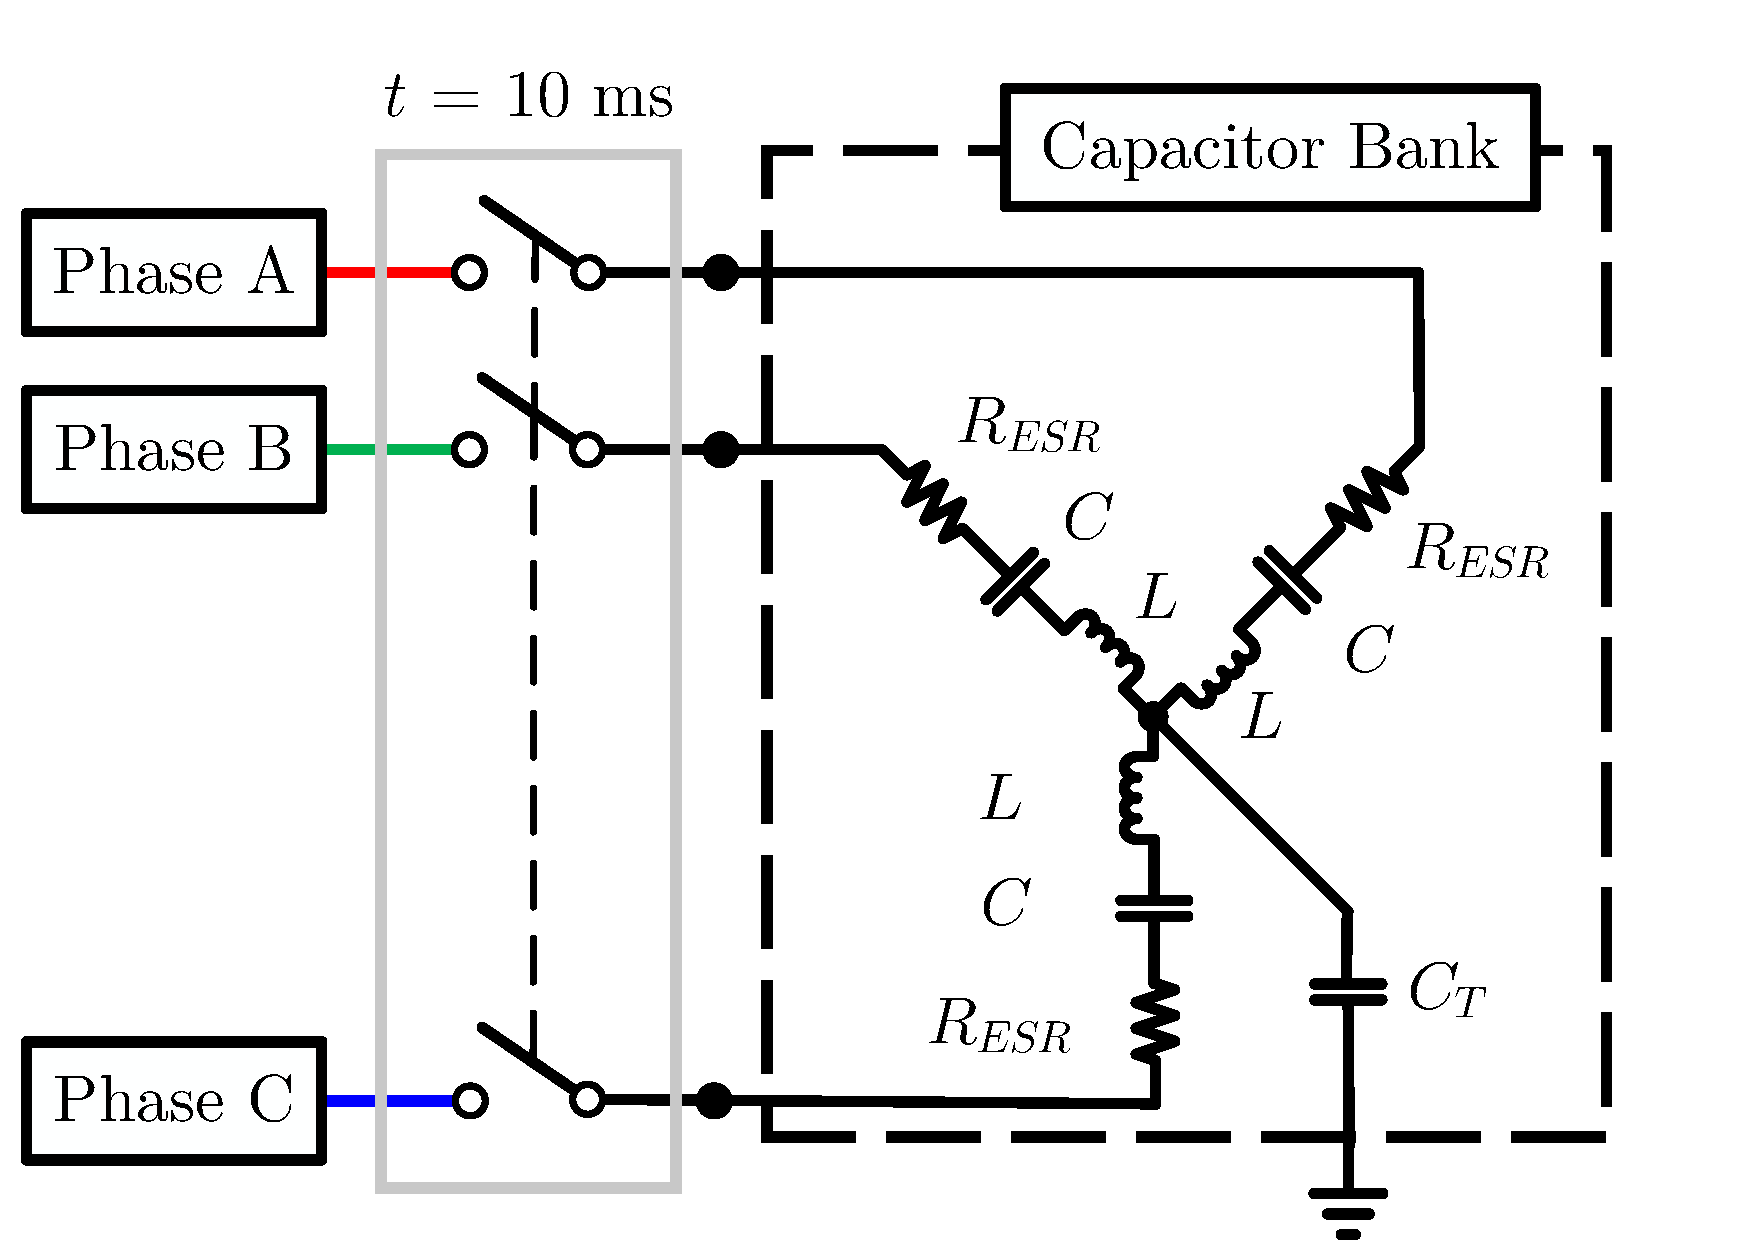
\includegraphics[width=8.4cm]{img/CapacitorBank.pdf}    % The printed column width is 8.4 cm.
		\caption{Capacitor bank diagram.} 
		\label{fig:CBdiagram}
	\end{center}
\end{figure}

Each CB branch is composed of inductances, resistances and capacitances. The intrisic inductance ($L$) represents the internal inductance and the current limiting reactor in the CB, whose value is 100 $\mu H$. $R_{ESR}$ is the internal resistance of the CB and represents losses in the components. A value of $R_{ESR} = 0.001$ $\Omega$ is considered. Finally, the capacitance ($C$) is calculated from nominal CB reactive power, whose value is 0.25 $\mu F$. The CB is connected to the ground through a capacitance ($C_{T}$) of 0.25 $\mu F$.

In Fig. \ref{fig:CBdiagram} is observed a three-phase switch, which start open and close at $t = 10$ ms. The charge switch is considered closed and the circuit operating in nominal load conditions before CB switch closure, as shown in Fig. \ref{fig:CBindVoltageTL}.

\begin{figure}[h]
	\begin{center}
		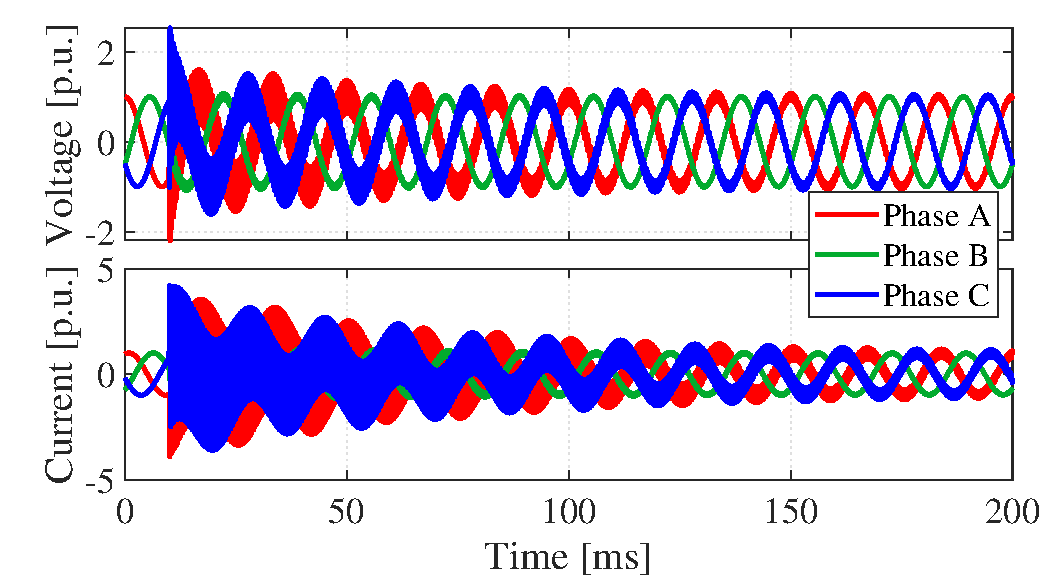
\includegraphics[width=8.4cm]{img/CBindVoltage_TL.pdf}    % The printed column width is 8.4 cm.
		\caption{Current and voltage waveforms at Terminal A for CB switching.} 
		\label{fig:CBindVoltageTL}
	\end{center}
\end{figure}

In instant of CB switch closure, induced voltage reaches its maximum value with 2.53 kV, as shown in Fig. \ref{fig:CBindVoltage}. Passing time of switch closure, the induced voltage magnitudes declines describing an exponential decay due to the action of capacitive coupling between the facilities, Fig. \ref{fig:CBindVoltage3plots} illustrates this performance. Induced voltage along pipeline has same behavior as under nominal load conditions in all time, differing in magnitudes. 

In steady-state after CB switching, induced voltage reaches 5.61 V.  

\begin{figure}[h]
	\begin{center}
		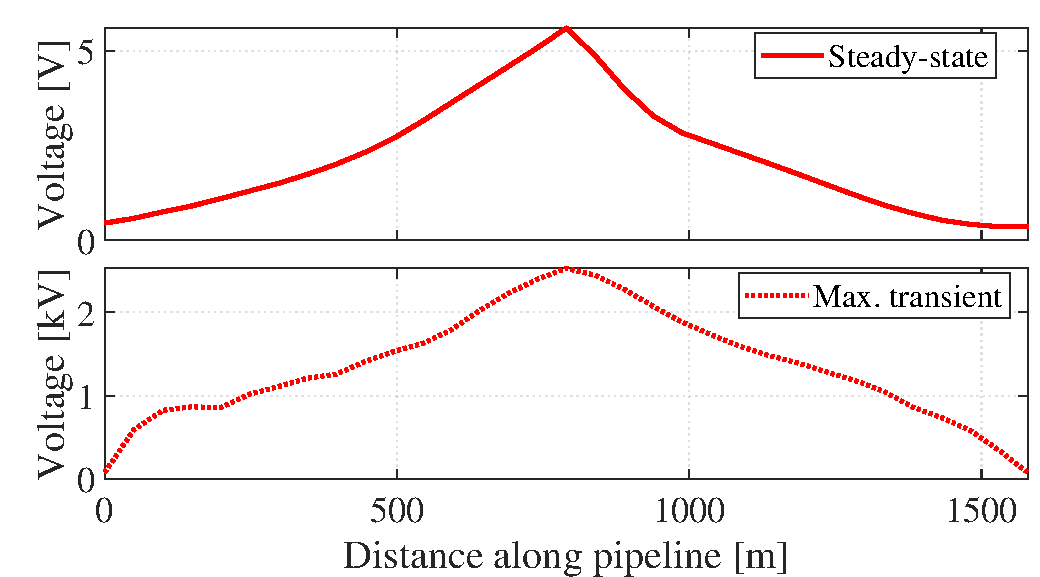
\includegraphics[width=8.4cm]{img/CBindVoltage.pdf}    % The printed column width is 8.4 cm.
		\caption{Steady-state induced voltage and maximum induced voltage along pipeline in CB switching.} 
		\label{fig:CBindVoltage}
	\end{center}
\end{figure}

\begin{figure}[H]
	\begin{center}
		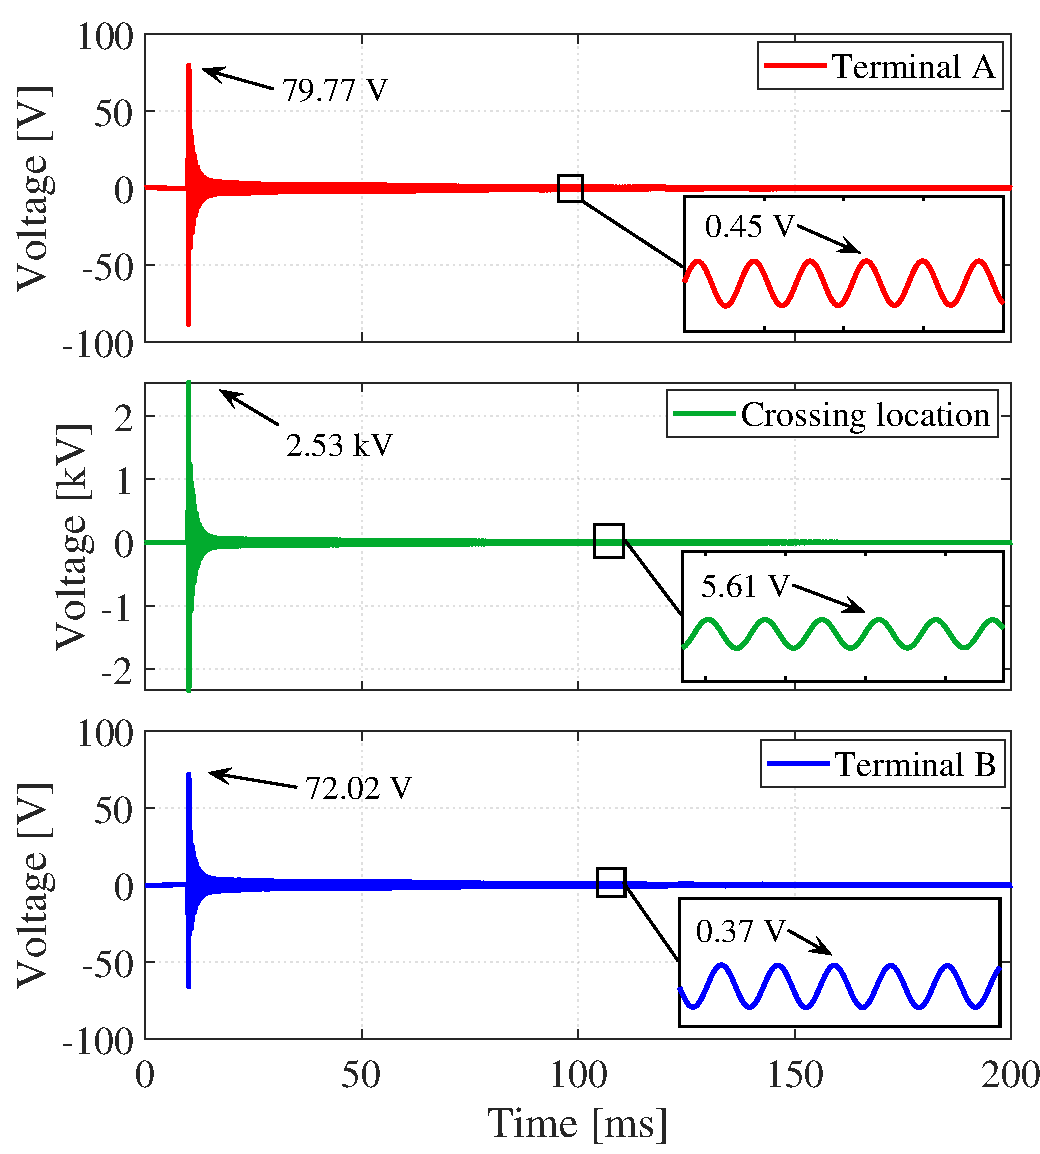
\includegraphics[width=8.4cm]{img/CBindVoltage_3plots.pdf}    % The printed column width is 8.4 cm.
		\caption{Induced voltage \textit{versus} time at Terminal A, Terminal B and nearby crossing location to CB switching.} 
		\label{fig:CBindVoltage3plots}
	\end{center}
\end{figure}

\section{Transmission line charge switching surges study}

For charge switching study, the system is considered in nominal load regime after charge switch closure. The charge switch starts opened and closes in 10 ms, as shown in Fig. \ref{fig:ENindVoltageTL}.

\begin{figure}[h]
	\begin{center}
		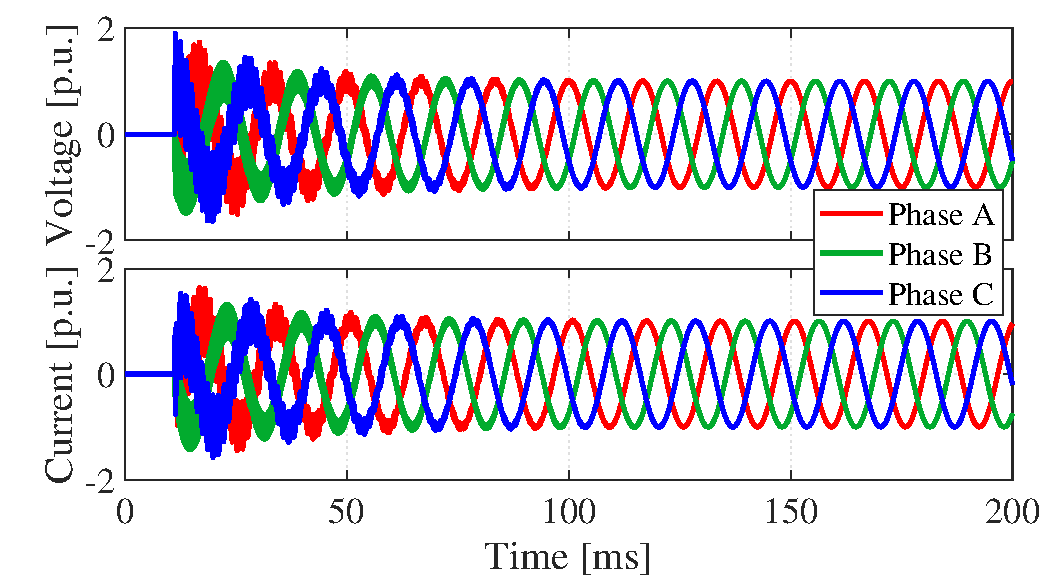
\includegraphics[width=8.4cm]{img/ENindVoltage_TL.pdf}    % The printed column width is 8.4 cm.
		\caption{Current and voltage waveforms at Terminal A for charge switching.} 
		\label{fig:ENindVoltageTL}
	\end{center}
\end{figure}

Voltage and current in TL reaches approximately 2 p.u. in transients regime.

\begin{figure}[h]
	\begin{center}
		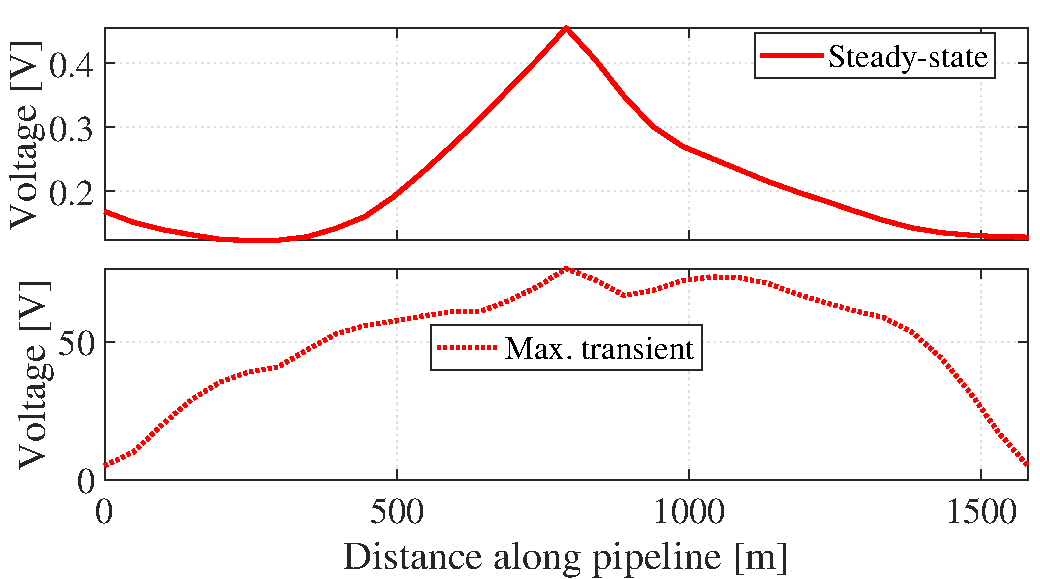
\includegraphics[width=8.4cm]{img/ENindVoltage.pdf}    % The printed column width is 8.4 cm.
		\caption{Steady-state induced voltage and maximum induced voltage along pipeline in charge switching.} 
		\label{fig:ENindVoltage}
	\end{center}
\end{figure}

In charge switching surges, transients regime is more relevant due to the fact in this time the induced voltage is higher than in nominal load conditions. Fig. \ref{fig:ENindVoltage} and \ref{fig:NLindVoltage3plots} shows that after transients regime the induced voltage returns to nominal load values.

\begin{figure}[h]
	\begin{center}
		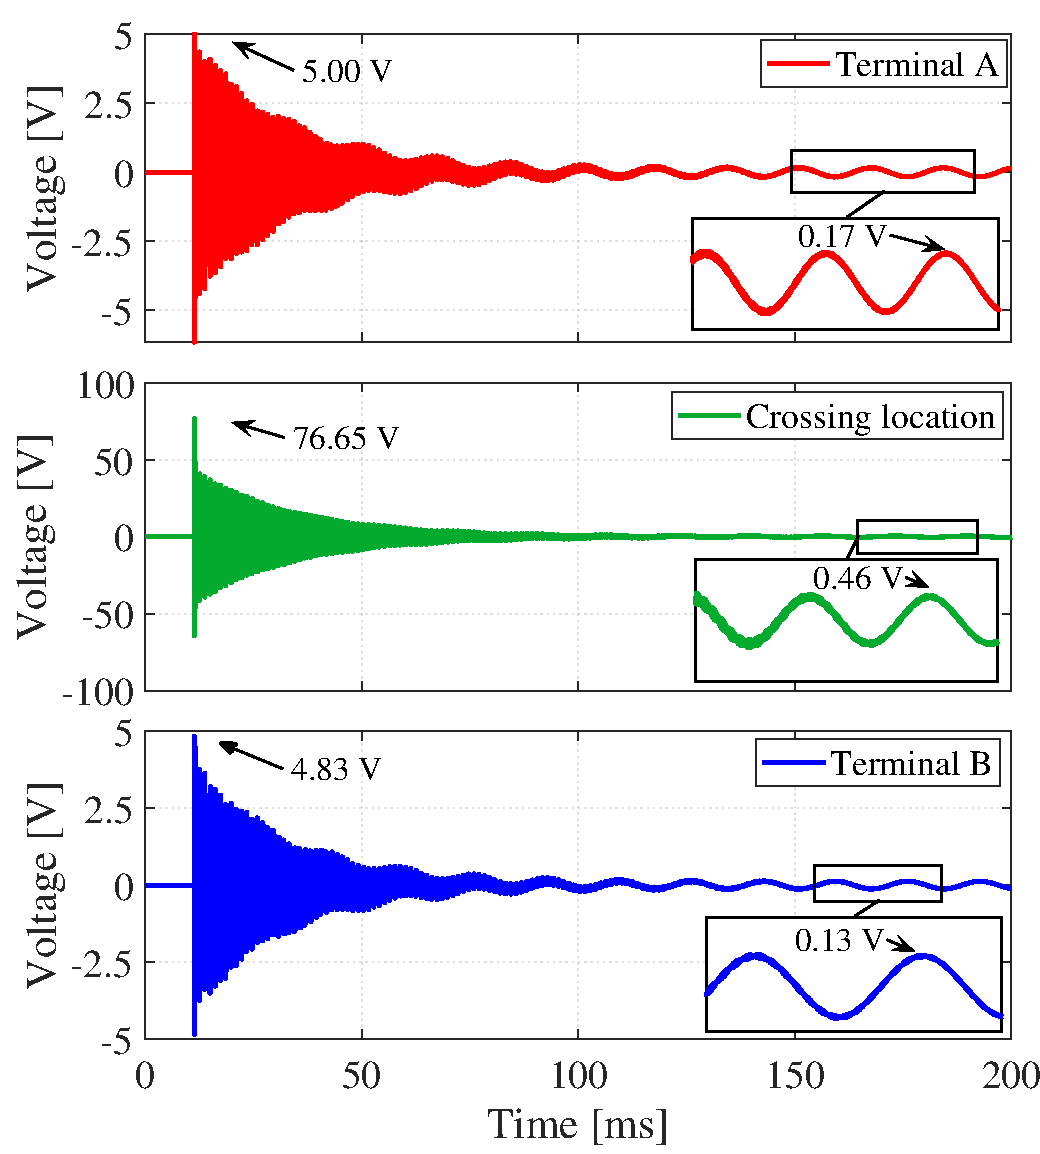
\includegraphics[width=8.4cm]{img/ENindVoltage_3plots.pdf}    % The printed column width is 8.4 cm.
		\caption{Induced voltage \textit{versus} time at Terminal A, Terminal B and nearby crossing location to charge switching.} 
		\label{fig:ENindVoltage3plots}
	\end{center}
\end{figure}



\section{Conclusions}

In this paper, inductive coupling interferences involving TL and nearby pipeline due to transients in the TL has been studied through a simple and precise circuit model. The analyzed system presented a shared right-of-way composed of arbitrary geometries. Switching surges and the mainly types of faults is applied to the TL.

The simulation results showed that the induced voltage and current on the pipeline can be much greater than the steady-state fault values, for all types of faults. 

In addiction, it was observed that the induced voltage is related with the unbalance factor in TL signal. For this reason, the voltage and current unbalance factor was calculated for each type of fault studied. The results presented a linkage between current unbalance and higher transients induced voltage. Also, greater unbalance signals in TL presents a greater pipeline induced voltage in steady-state fault regime. Result shows that faults involving soil was the worst for the system presenting higher unbalance signals in TL and induced voltage in transient and steady-state fault regime.

Capacitor bank switching surges presents that induced voltage waveforms are influenced by capacitor discharging due to capacitive coupling between TL and pipeline and the induced voltage has the same behavior in all time, just decaying in magnitudes exponentially.

Results in charge switching surges, presents that the transient regime is most relevant. In transients regime, induced voltage increases but, with the passing time, induced voltage returns to nominal load magnitudes. Then, the transient regime presents the risks for installations in shared right-of-way.


\bibliography{library}

\end{document}